\chapter{Textual Data}
\label{chap:textual-data}
Integrating data, particularly newspaper article content is a fundamental component of our application. To ensure a sufficient implementation, we must consider several aspects. The following chapter will discuss these aspects from different perspectives, including the developer's viewpoint and legislative considerations.

Using full text maximises the potential and value of the data, but this complicates the development of an application based on historical and current data. The chapter further states that static datasets are unsuitable for our application and emphasises the need to select a source that provides both historical and current data. The chapter also focuses on terms of service because of recent legal disputes between the New York Times, Microsoft and OpenAI, highlighting the importance of adhering to these rules when using data resources.

Various data extraction techniques, such as \acrshort{rss} feeds, web scraping, and \acrshort{api}, are discussed from the perspective of using them for the development and reliability of our application. Each method has its advantages and disadvantages, which are further elaborated. The chapter mainly focuses on \acrshort{api}s, preferred when provided directly by data sources. They provide good quality and reliable data, although third parties may offer alternative solutions with some limitations, which are discussed. The experiments performed in this chapter are available in the attached Python notebook\footnote{Located in the directory /ipynbs/textual-data/.}.

At the end of the chapter, we decided that the Guardian was the most appropriate source and, because obtaining other data was unattainable, our only source. We have also decided that the timeframe we have set is three months, and due to the data's lifecycle, we have to remove all data from the database every $24$ hours at most.

\section{Introduction}
\label{chap:textual-data-introduction}
In the context of entity-level sentiment analysis, it is essential to retrieve the entire textual content of each article. The internet holds vast amounts of information, making it more reasonable to obtain the content of an article rather than just its headline. The full text contains all the entities concerned, whereas the headline may not include all mentioned entities. Consequently, this allows us to maximise the potential and value of data such as news articles. This requirement complicates the development process from the beginning. Building an application on a dataset from the past would be inefficient as it would not include current news coverage, making it useless to the user. Therefore, we address this data retrieval process in the following sections. We aim to find a source that provides both historical and current data. Therefore, we will not consider static datasets as a data source for the deployed application. When selecting a data source for news article content, it is essential to consider the following aspects:

\begin{description}
    \item[Reliability] Expresses the degree to which data sources can be trusted based on their history and reputation.
    \item[Availability] Refers to the availability of the news articles for our application and factors such as the cost of the data.
    \item[Accessibility] Refers to the ease with which data source can be accessed. Consider data retrieval methods and any restrictions on accessing news articles.
    \item[Consistency] Stands for the data source that maintains a consistent format and structure, facilitating easier integration into our application.
    \item[Terms of Service] Considers the terms of service of the data source, which define the rules and regulations for using the data source.
\end{description}

Before we get to these and delve into specific extracting techniques and data sources, where we will elaborate on these aspects, we are devoting a separate section to the terms of service aspect due to recent events.

\section{Terms of Services}
\label{sec:textual-data-terms-of-services}
When integrating data such as news articles into an application, it is essential to consider the data source's terms of service. The terms of service define the rules and regulations we must follow when using the data. These terms include restrictions on use and lifecycle. Complying with the terms of service is crucial because violating these rules may lead to blocked access to data or lawful problems. The impetus for including this section is a recent dispute initiated by the New York Times, which filed a lawsuit against Microsoft and OpenAI \parencite{Stempel2023, Bergen2023}.

Although our application does not use generative artificial intelligence, which is the cause of this dispute, the data use terms for most providers cover machine learning models in their entirety. These terms are often mentioned in the context of data used for training models. Data providers are concerned that their data is being used to train models that may lead off readers who could be subscribers to their paid content or miss out on monetary gains from advertising. The New York Times was concerned that chatbots like ChatGPT and Copilot from the companies mentioned above used direct excerpts from their articles in the responses from their generative models.

The dispute initiated by the New York Times was directed towards regulating the use of their data to train models and delineating the damages that were incurred due to the breach of the agreement between the companies and the New York Times. This litigation certainly has implications for the future use of data from other newspaper resources, not just Microsoft and OpenAI. Therefore, it is essential to pay attention to this matter. The New York Times was the first major US media organisation to raise the issue. In April of this year, eight newspapers owned by Alden Global Capital made further allegations against Microsoft and OpenAI \parencite{Robertson2024, Associated_Press2024}.

With this section, we want to emphasise that we can not arbitrarily use data such as articles. They are subject to copyright, and most companies make legitimate attempts to protect this data from unauthorised use, which we cannot ignore.

\section{Data Extraction Techniques}
\label{sec:textual-data-harvesting-approaches}
Different approaches to data extraction exist. In our case, we focus on the possibility of extracting textual data as whole content from newspaper articles. This section looks at several basic methods for extracting text data from news articles, including web scraping, \acrfull{rss} feeds \parencite{rssmarco}, and \acrfull{api}. We intentionally omit static datasets in the following subsections because they do not provide recent information.

\subsection{RSS Feeds}
\label{sec:textual-data-rss-feeds}
One of the oldest approaches for obtaining data is Really Simple Syndication, also known as \acrshort{rss}. It is a standard used to provide updated content on web pages. These feeds are typically used to provide breaking news, blogs, and other information on the internet. It uses XML format and typically contains headlines, descriptions, and link information to the article. \acrshort{rss} feeds are, in most cases, provided only by section and include $20$ to $100$ new articles over a while, typically a day to a week. This is insufficient as we need control over the actual specifications for this period. 

The feeds with direct article content are impossible to find in official and well-known sources such as the New York Times, Bloomberg, Reuters, and more. This choice of data would be ideal if we were primarily looking for updates to a data source without the possibility of obtaining historical data within the specified time range. In that case, consider the successor to \acrshort{rss}, namely the Atom Syndication Format \parencite{atom-wiki} standard for feeds. However, it still needs to address the necessity for historical data, and we have also been searching for an official channel that provides the entire content but unsuccessful. Therefore, we omit \acrshort{rss} feeds when evaluating individual sources.

\subsection{Web Scraping}
\label{sec:textual-data-web-scraping}
Another option is web scraping, which involves extracting data from web pages. This approach is subject to limitations defined by the Robots Exclusion Protocol (REP) in a text file called \textit{robots.txt}. This file is typically located in a website's root directory and contains rules for programs, such as robots. It determines whether the page can be crawled, a standard process associated with web scraping. 

Given the number of requests needed to obtain the full content of several articles, web scraping is unsuitable for our application. We would have to crawl all the pages of all articles and extract all the text content from them. One disadvantage of this approach is the potential blocking of the IP address, which could result in being denied access to the data, as it is not an official method for accessing the data that websites require. This is one of the reasons why websites try to regulate crawling using \textit{robots.txt} for ethical crawling and scraping. However, it is essential to realise that REP does not grant us access to the data. It simply specifies the rules we should follow when crawling the pages.

Another disadvantage is the data quality and reliability we can obtain this way. The data's consistency and structure are also problematic because each website has a different structure. We would have to create a specific web scraper for each source, which is challenging and inefficient. Compared to other obtaining data techniques, such as \acrshort{api}, creating a scraper is much less efficient and demanding in terms of development, especially in terms of maintenance. However, we would use this approach, for example, if we wanted to source from a blog or news source that does not provide an official \acrshort{api}. In addition, we use this approach rather than \acrshort{rss} feeds because it allows us to access both historical and current data.

\subsection{API}
\label{sec:textual-data-api}
Application Programming Interface, also known as \acrshort{api}, is a collection of defined rules and protocols allowing software applications to communicate. It serves an interface that facilitates communication between the data source and our application by querying existing endpoints. \acrshort{api}s are complemented by documentation that details how to use the \acrshort{api}, which endpoints are available, what parameters can be used, and what limitations apply. \acrshort{api} providers typically offer plans that determine how many queries we can complete in a given period or impose other limitations. We distinguish between \acrshort{api}s provided directly by the data source and those provided by third parties.

In the first case, we might use \acrshort{api}s from providers such as The New York Times\footnote{\href{https://www.developer.nytimes.com/apis}{https://www.developer.nytimes.com/apis}}, Bloomberg\footnote{\href{https://www.bloomberg.com/professional/products/data}{https://www.bloomberg.com/professional/products/data}}, Reuters\footnote{\href{https://www.liaison.reuters.com}{https://www.liaison.reuters.com}}, and others. \acrshort{api}s provided directly by the data source are usually the best choice because they provide direct access to the data and naturally have the highest quality. These \acrshort{api}s typically offer endpoints that allow us to retrieve entire articles, though it remains a question whether they are available in a paid plan or for free. %todo kdyztak hodit do citace

Third-party \acrshort{api}s can be helpful if we do not have access to an \acrshort{api} provided directly by the data source or want to combine data from various sources with less effort. However, third-party \acrshort{api}s may have limitations that can affect data quality, such as incomplete or inconsistent data, since they provide data from many sources\footnote{They may include sources offering their \acrshort{api}s as primary providers.}, which can lead to vaguely defined specifications and data inconsistency, for example as information about what the articles sections contain.

Due to the variability of \acrshort{api}s from specific providers, we will divide our discussion into two separate sections. The first section will focus on third-party data providers, and the second will delve into first-party data providers.

\section{Third-party Data Providers}
\label{sec:textual-data-third-party-data-providers}
%https://newsdata.io/documentation
Third-party \acrshort{api}s provide article data aggregated from various sources on the internet. Since they are available in different pricing plans and we have not noted any exceptions for research purposes, we will focus only on free plans. Thus, we are subject to the most common limitation, the maximum number of queries within a specified period. Most providers offer free plans, primarily allowing developers to test various endpoints and verify if they meet the application's requirements. The number of allowed queries with this type of provider is meagre, typically ranging from $10$ to $20$, with not many articles in response. The data also contains limitations with a delay of $12$ - $24$ hours, as seen with NewsData\footnote{\href{https://www.newsdata.io/}{https://www.newsdata.io/}}.

In our application, we would likely be able to limit the number of queries to still use the free plan without losing access to the required endpoints. Of course, we could use \acrshort{api}s providing sentiment analysis, such as Alpha Vantage\footnote{\href{https://www.alphavantage.co}{https://www.alphavantage.co}}. However, none of these providers provide information about the models and calculations they use, which we do not consider suitable given the nature of this thesis. We have attempted to contact several providers but have not received a response.

During our examination of various \acrshort{api}s, we consistently encountered a common issue: incomplete or misunderstood service specifications. To illustrate this concern, we present an example within the context of news article \acrshort{api}s. Although Finnhub\footnote{\href{https://www.finnhub.io}{https://www.finnhub.io}} does not provide full-text content article data, we also tried an endpoint that includes purely articles within the given company during testing. While Finnhub does not impose strict limits on query volume, its website indicates a maximum of 60 \acrshort{api} calls per minute under the free plan.

Finnhub's documentation \parencite{finnhub_doc} claims to offer ``\textit{1 year and real-time updates}'' within its fundamental data services. Its company news endpoint allows developers to specify parameters such as \textit{from} and \textit{to} for retrieving data within specific periods. Developers like us may request data from the past month, which could be, from a particular perspective, qualified as the latest data. However, how many articles or days of data are included within this timeframe remains unclear, highlighting a need for more transparent specifications and validation. We conducted tests using the Finnhub \acrshort{api} for the last two quarters of $2023$ and the first quarter of $2024$, focusing on companies such as Apple Inc. (AAPL), Microsoft Corp. (MSFT), Alphabet Inc. (GOOGL), and Amazon.com Inc. (AMZN). The volume of articles for individual quarters, distributed across individual days, is shown in Figure \ref{fig:finnhub-q1-2024} and those attached in Appendix \ref{appsec:third-party-data-providers}.

\begin{figure}[htbp]
    \centering
    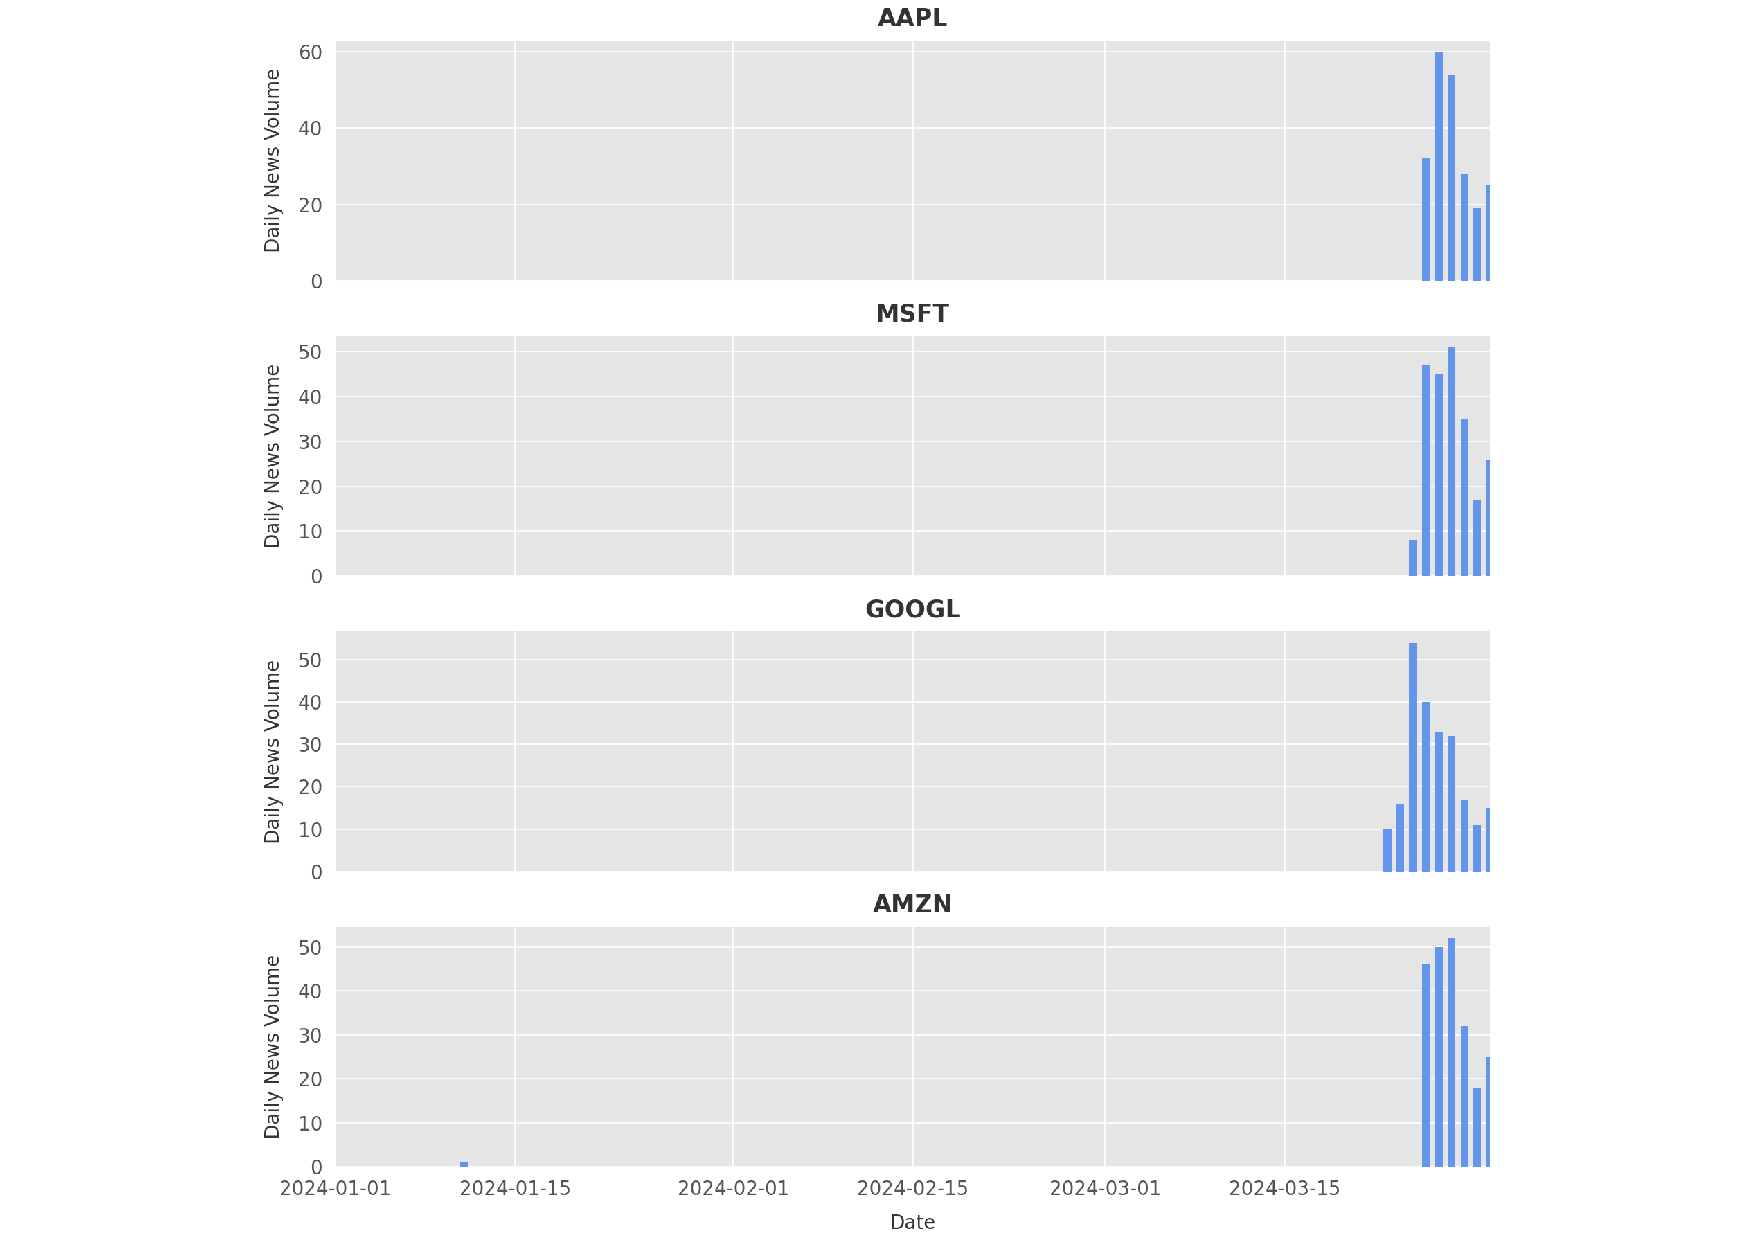
\includegraphics[width=\textwidth]{img/textual-data/q1-2024-a.pdf}
    \caption{Finnhub daily news articles volume of Apple Inc. (AAPL), Microsoft Corp. (MSFT), Alphabet Inc. (GOOGL), and Amazon.com Inc. (AMZN) for the first quarter of 2024}
    \label{fig:finnhub-q1-2024}
\end{figure}

We have not even identified a consistent pattern to guide the data, so it is unclear what exactly the latest fundamental data means, even though we can set the range parameters \textit{from} and \textit{to} for the past year. In addition, Figure \ref{fig:finnhub-q1-2024} illustrates an article at Amazon.com on January $11$th, early in the first quarter of $2024$, highlighting the data's inconsistency. It is not our goal to cast a pall over Finnhub but only to point out a shortcoming that is also present in other third-party providers within the specification.

Analysing each third-party resource is a time-consuming process that complicates the development of our proposed application due to misleading \acrshort{api} specifications. Moreover, we are uncertain if all third-party providers have proper permissions to acquire data by the terms of service of the original data providers. With data from numerous newspapers, determining liability in potential legal issues remains ambiguous. Additionally, the extent to which we should adhere strictly to the terms established by third parties or direct data sources remains unclear.

\section{First-party Data Providers}
\label{sec:textual-data-first-party-data-providers}
First-party data providers are the ideal choice. Typically, the \acrshort{api} specifications of these providers differ in minor ways, but they can provide quality and reliable results. We have reviewed many sources that might be suitable for our application. Reuters and Bloomberg do not provide a free plan allowing us to extract entire articles. The New York Times provides a free \acrshort{api}, but it does not have the ability to extract entire articles. We must request a modified data solution to extract this data, which is almost impossible for free. We further attempted to obtain data from the Financial Times. However, they were unable at the time of our investigation to handle the volume of requests they receive from the students and faculty for accessing their \acrshort{api}. Ultimately, the only one who provided us access to its data is the Guardian through its platform, the Guardian Open Platform\footnote{\href{https://www.open-platform.theguardian.com}{https://www.open-platform.theguardian.com}}.

The Guardian is a British daily newspaper that covers news across the world. Through its official Open Platform, the Guardian provides a free \acrshort{api} that allows us to extract articles, including entire textual content. After describing our research and thesis objectives to the Guardian, we accessed its complete \acrshort{api}, allowing us to retrieve full-text articles with a daily limit of $500$ \acrshort{api}  calls. This is sufficient for us as it provides an endpoint for searching by section, where the default result of the number of articles per response page is $10$. However, this parameter can be changed to $200$, whereby we can retrieve $200$ articles per query. An additional benefit is the capability to retrieve data for the current day.

Our study will focus on a three-month timeframe, explicitly exploring the business and technology sections. However, following their condition, which is that the data lifecycle must be less than $24$ hours, is essential. This means we must remove the data from the database every $24$ hours. For these reasons and other capacity constraints, we chose a time frame of three months to process the data, and we see this as sufficient time for our needs.

To compare the daily volume of news articles with third-party data providers, we conducted a comparative experiment using data from the Guardian as a first-party data provider. Unlike Finnhub, which uses direct ticker references, we utilised literal mentions querying of companies. The results from The Guardian are illustrated in Figure \ref{fig:guardian-q1-2024} and those attached in Appendix \ref{appsec:first-party-data-providers}.

\begin{figure}[htbp]
    \centering
    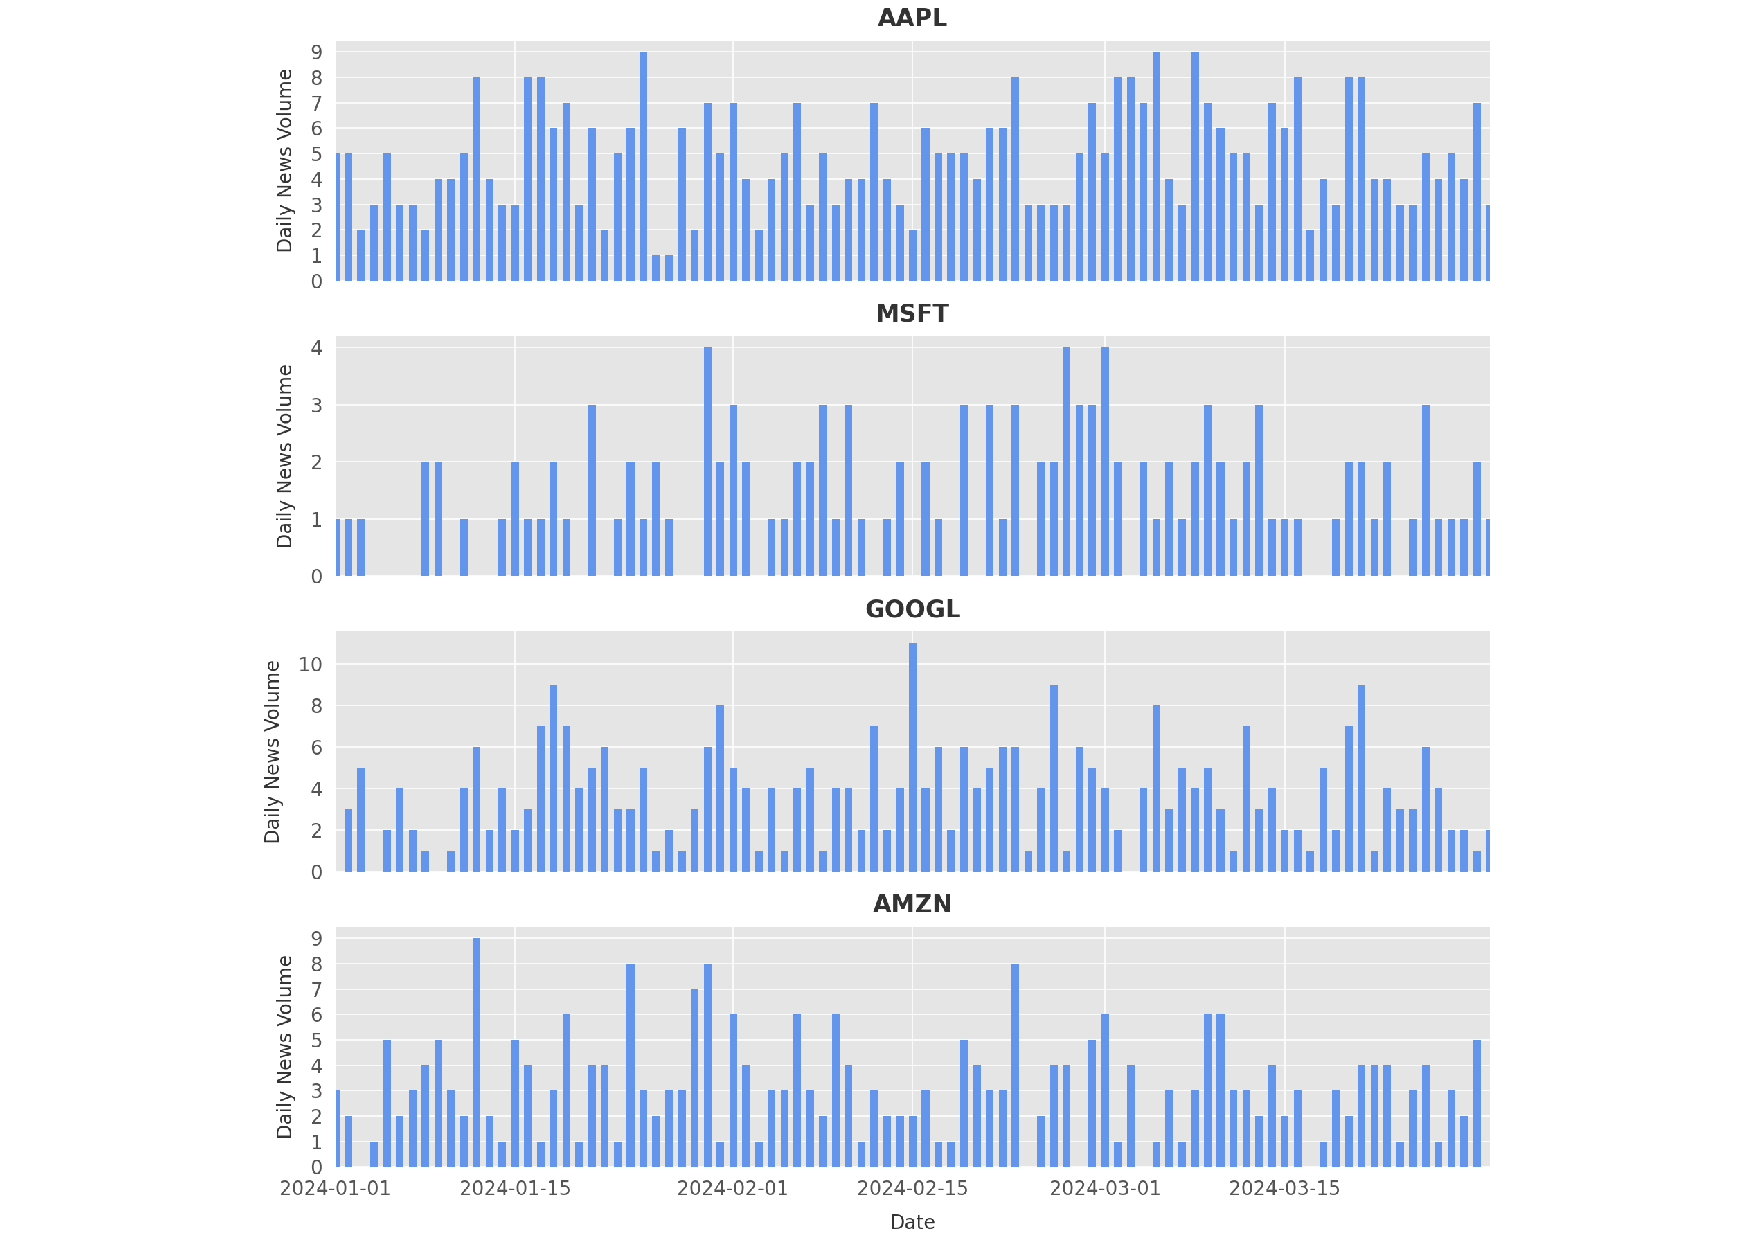
\includegraphics[width=\textwidth]{img/textual-data/guardian-q1-2024-a.pdf}
    \caption{The Guardian daily news articles volume of Apple Inc. (AAPL), Microsoft Corp. (MSFT), Alphabet Inc. (GOOGL), Amazon.com Inc. (AMZN) for the first quarter of 2024}
    \label{fig:guardian-q1-2024}
\end{figure}

First-party data providers proved preferable, providing comprehensive data quality and reliability as direct sources. This approach enables us to obtain data that accurately reflects reality while ensuring compliance with the terms of service to avoid legal issues. After explaining the thesis's purpose and intentions for data usage, the \acrshort{api} key was provided to us. We extend our gratitude to Guardian for providing us with the data for research and implementation in this thesis, as procuring such a data source was very challenging. Reflecting on the aspects discussed earlier in this chapter, the Guardian is an ideal choice for our application as a first-party data provider. Its data is of outstanding quality, reliable, and efficiently accessible, and we fully comply with the terms of service.